\documentclass[11pt,a4paper]{article}

\usepackage[spanish,es-nodecimaldot,es-tabla]{babel}
\usepackage[utf8]{inputenc}
\usepackage[T1]{fontenc}
\usepackage{lmodern}
\usepackage[margin=2.5cm]{geometry}
\usepackage{amsmath,amssymb}
\usepackage{graphicx}
\usepackage{booktabs}
\usepackage{siunitx}
\usepackage{subcaption}
\usepackage{xcolor}
\usepackage[hidelinks]{hyperref}
\usepackage[style=ieee,backend=biber]{biblatex}

\sisetup{output-decimal-marker={,}}
\graphicspath{{figuras/}}
\addbibresource{bibliografia.bib}

% Marca lo que falta completar. Para la entrega: \renewcommand{\pendiente}[1]{}
\newcommand{\pendiente}[1]{\textcolor{red}{[#1]}}

\begin{document}

\begin{titlepage}
\centering

\includegraphics[width=0.4\textwidth]{logo_itba}\par\vspace{1cm}
{\Large Instituto Tecnológico de Buenos Aires\par}
\vspace{0.5cm}
{\large Procesamiento de Señales e Imágenes Biomédicas (16.63)\par}
{Comisión BIO\par}
\vspace{2cm}
{\huge\bfseries Informe final\par}
\vspace{0.5cm}
{\Large Clasificación automática de estadios de sueño\\a partir de la polisomnografía\par}
\vspace{0.3cm}
{Trabajo Práctico de Señales (TPS)\par}
\vspace{2cm}
{\bfseries Grupo 2\par}
\vspace{0.3cm}
65555 -- Cassano Nieto, Facundo Tomás (\href{mailto:fcassanonieto@itba.edu.ar}{fcassanonieto@itba.edu.ar})\par
65414 -- D'Elía, Lucas Valentín (\href{mailto:ldelia@itba.edu.ar}{ldelia@itba.edu.ar})\par
65560 -- Ortega, Facundo (\href{mailto:facortega@itba.edu.ar}{facortega@itba.edu.ar})\par
\vspace{1.5cm}
{\bfseries Docentes\par}
\vspace{0.3cm}
Tomás, Roberto Sebastián\par
Capurro, Lucila\par
Reppucci, Victoria\par
Tassara, Francisco Joaquín\par
\vfill
{10 de noviembre de 2026\par}
\end{titlepage}


\begin{abstract}
\pendiente{Resumen de 150 a 200 palabras: problema, método, $\kappa$ obtenido y conclusión principal.}
\end{abstract}

\tableofcontents
\newpage

\section{Introducción}
% Base: sección 1 del anteproyecto. Pasar a pasado lo que ya se hizo.

\subsection{Problemática}
La polisomnografía (PSG) es el estudio de referencia para diagnosticar trastornos del sueño: durante una noche se registran en simultáneo EEG, EOG, EMG de mentón y ECG. Según el manual de la AASM~\cite{berry2017}, el registro se divide en épocas de \SI{30}{\second} y a cada una se le asigna uno de cinco estadios: vigilia (W), sueño ligero (N1 y N2), sueño profundo (N3) o sueño REM. La secuencia de estadios de toda la noche se denomina hipnograma.

Esta clasificación la hace un técnico a mano, época por época, y el resultado depende de quién la haga. Entre técnicos de distintos centros se reportó $\kappa = 0{,}76$~\cite{dankerhopfe2009} y entre los técnicos del Haaglanden Medisch Centrum (HMC), $\kappa = 0{,}74$~\cite{alvarez2021}. N1 es el estadio en el que menos coinciden.

\subsection{Marco teórico}
\pendiente{Frente A y B: qué aporta cada señal y artefactos (anteproyecto §1.2).}

\subsection{Estado del arte}
\pendiente{Anteproyecto §1.3: descriptores + clasificador (YASA~\cite{vallat2021}) frente a redes profundas~\cite{alvarez2021}.}

\subsection{Objetivos e hipótesis}
\textbf{Objetivo general.} Desarrollar un algoritmo sin técnicas de inteligencia artificial que clasifique cada época de una PSG en uno de los cinco estadios, con decisiones explicables a partir de las señales, que alcance un acuerdo con los técnicos cercano al que tienen entre sí ($\kappa \approx 0{,}74$), junto con una interfaz gráfica que muestre cada etapa del procesamiento.

\textbf{Hipótesis.}
H1, el espectro multitaper varía menos que el de Welch entre épocas de un mismo estadio;
H2, el promediado de Woody recupera la forma de la onda lenta con menor error que el promedio ordinario y ayuda a separar N2 de N3;
H3, los descriptores CSP mejoran la clasificación de N1 y REM;
H4, quitar los artefactos y agregar la HRV mejora el acuerdo con los técnicos.

\section{Materiales y métodos}

\subsection{Base de datos}
Se usó la HMC Sleep Staging Database v1.1~\cite{alvarez2022}, con 151 PSG de adultos registradas a \SI{256}{\hertz}, con cuatro canales de EEG (F4, C4, O2 y C3, referidos a la mastoide contralateral), dos de EOG, EMG de mentón y ECG, anotados por técnicos según la AASM. Se eligieron al azar 70 registros con una semilla fija y se separaron por paciente en 56 de entrenamiento y 14 de prueba. Todos los parámetros se eligieron con los pacientes de entrenamiento. La clasificación y la evaluación se restringieron a las épocas entre las marcas de luces apagadas y encendidas, porque la vigilia fuera de ese período es fácil de clasificar y corre hacia W la mediana de la noche con que se normalizan algunos descriptores (Sección~\ref{sec:clasificacion}). El código está en Python y los archivos del repositorio se describen en el Anexo~\ref{sec:archivos}.

\subsection{Preprocesamiento}
\textbf{Exploratorio y filtrado.} En el espectro crudo de cada canal se midió cuánto sobresalen 50 y \SI{60}{\hertz} respecto de sus vecinas, y del encabezado EDF se leyó el rango físico (\SI{\pm800}{\micro\volt} en el EEG) y los filtros del equipo, un pasa-altos de \SI{0,2}{\hertz} y un pasa-bajos de 35 o \SI{128}{\hertz} según el registro. El EEG y el EOG se filtraron con un pasa-altos de \SI{0,2}{\hertz}, un pasa-bajos de \SI{45}{\hertz} y un notch de \SI{50}{\hertz}, y el EMG con un pasa-altos de \SI{10}{\hertz} y el notch. El pasa-altos bajó respecto de los \SI{0,5}{\hertz} del anteproyecto para no recortar las ondas lentas. Se comparó un IIR Butterworth de orden 4 aplicado hacia adelante y hacia atrás con un FIR por ventana de Hamming, y se adoptó el IIR porque da la misma forma de onda con orden 4 en lugar de 4225 coeficientes.

\textbf{Artefacto ocular.} Con E1$-$E2 como referencia se compararon NLMS y el filtro de Wiener, ambos filtros óptimos. Como la referencia también contiene ondas lentas cerebrales, se agregó una compuerta para que el filtro se ajuste y se aplique solo donde el valor eficaz del EOG en \SI{2}{\second} supera el doble de su mediana de la noche. Las variantes se compararon en F4 con la potencia delta y las ondas lentas detectadas por estadio, que deberían bajar en W y REM y no cambiar en N3.

\textbf{Latidos y artefacto cardíaco.} Los latidos se detectaron con Pan-Tompkins~\cite{pan1985} (pasa-banda de 5 a \SI{15}{\hertz}, derivada, cuadrado, integración en \SI{150}{\milli\second} y umbrales adaptativos), con la polaridad decidida una vez por noche y los umbrales reiniciados tras \SI{5}{\second} sin latidos. Para ver si el artefacto cardíaco era relevante, como pidió la cátedra, se promedió el EEG entre $-0{,}2$ y \SI{0,6}{\second} alrededor de cada onda R, donde el EEG se cancela y el artefacto se conserva, con un control en instantes al azar. Para removerlo, en cada latido se restó el promedio de los 30 latidos anteriores, sin las ventanas de más de \SI{500}{\micro\volt} pico a pico.

\textbf{Segmentación.} Siguiendo la devolución, se analizaron épocas fijas de \SI{30}{\second}. Para marcar las que mezclan dos estados se ajustó un modelo AR de orden 8 (Yule-Walker) en los primeros \SI{5}{\second} de cada época de C4 y se aplicó a los cinco tramos siguientes. La época se marcó como no estacionaria si el error de predicción de algún tramo superaba 4 veces al del primero. La marca no interviene en la clasificación.

\subsection{Descriptores}
\textbf{Espectro multitaper.} El periodograma de una época tiene un error del orden de su propio valor. Welch~\cite{welch1967} lo reduce promediando tramos más cortos, mientras que el multitaper~\cite{thomson1982,prerau2017} usa la época completa multiplicada por $K$ ventanas de Slepian ortogonales y promedia los $K$ espectros, casi independientes, con lo que la varianza baja unas $K$ veces. Con $NW = 15$ la resolución es de \SI{1}{\hertz} y se usaron $K = 2NW - 1 = 29$ ventanas. Para H1, Welch se calculó con ventanas de Hann de \SI{4}{\second}, también de \SI{1}{\hertz} de resolución. Por canal se calcularon la potencia de $\delta$, $\theta$, $\alpha$, $\sigma$ (\SIrange{11}{16}{\hertz}) y $\beta$ (\SIrange{13}{30}{\hertz}) en logaritmo y como fracción de la potencia entre 0,5 y \SI{30}{\hertz}, los cocientes $\delta/\theta$, $\delta/\beta$ y $\theta/\alpha$ y la pendiente del espectro en escala log-log entre 1 y \SI{40}{\hertz}~\cite{donoghue2020}, 56 descriptores en total.

\textbf{Husos, ondas lentas y Woody.} Los husos se detectaron en C4~\cite{molle2002} filtrando entre 11 y \SI{16}{\hertz}, con la envolvente de Hilbert suavizada en \SI{0,2}{\second} y un umbral de la media más 1,5 desvíos de la envolvente de la noche, durante 0,5 a \SI{2}{\second}. Las ondas lentas se detectaron en F4 con el criterio visto en clase~\cite{piantoni2013}, filtrando entre 0,2 y \SI{4}{\hertz} y aceptando las ondas con pico negativo menor a \SI{-60}{\micro\volt} y al menos \SI{75}{\micro\volt} pico a pico. Para estimar la forma típica de las ondas de cada paciente se recortó cada una \SI{\pm1}{\second} alrededor de su pico. Como el ruido corre el pico detectado, el promedio ordinario mezcla ondas desalineadas. El método de Woody~\cite{woody1967} parte de ese promedio, busca para cada onda el corrimiento de hasta \SI{0,25}{\second} que maximiza su correlación cruzada con la plantilla, recalcula la plantilla y repite, con un máximo de 20 iteraciones. Por época se guardaron la cantidad y amplitud de husos y de ondas, y el parecido medio de las ondas con la plantilla.

\textbf{CSP.} Los patrones espaciales comunes~\cite{ramoser2000} buscan una combinación de los cuatro canales, $s = \mathbf{w}^\top\mathbf{x}$, con mucha potencia en un estadio y poca en otro. Se aplicaron al par N1 y REM, el que más se confunde. Con las covarianzas medias de entrenamiento de cada estadio, normalizadas por su traza, se resolvió $\mathbf{C}_{N1}\mathbf{w} = \lambda(\mathbf{C}_{N1}+\mathbf{C}_{R})\mathbf{w}$, se conservaron los dos autovectores de cada extremo y el descriptor fue $\log(\mathbf{w}^\top\mathbf{C}\,\mathbf{w})$ de cada época.

\textbf{EOG, EMG y HRV.} Del EOG se usó la energía de E1$-$E2 por época, donde los movimientos oculares se refuerzan y la actividad cerebral se cancela, y del EMG su valor eficaz, ambos en logaritmo. Para la HRV se descartaron los latidos con correlación menor a 0,8 con el latido típico de la noche (la mediana de todos), y después los intervalos RR fuera de 0,3 a \SI{2}{\second} o a más de un 20\,\% de la mediana de sus vecinos. Como la serie queda con muestras irregulares, el espectro se estimó con el periodograma de Lomb en una ventana de \SI{5}{\minute} centrada en cada época, y se guardaron el logaritmo de HF y de LF/HF~\cite{taskforce1996}.

\subsection{Clasificación}
\label{sec:clasificacion}
El anteproyecto proponía un LDA y un HMM, pero la devolución aclaró que la clasificación no puede usar inteligencia artificial, y ambos se entrenan con épocas etiquetadas. Se los reemplazó por reglas construidas a partir del manual AASM~\cite{berry2017} y un suavizado con reglas fijas, lo que además deja cada decisión explicada por una regla concreta.

Las potencias relativas se usaron como fracción y los husos y ondas como conteo por época, magnitudes que no dependen de la amplitud del registro. El EMG, el EOG y LF/HF sí dependen del paciente y se expresaron como múltiplo de la mediana de su noche, $10^{\,x-\operatorname{mediana}(x)}$. Una primera versión con todos los descriptores en percentiles de la noche dio $\kappa = 0{,}245$, porque un umbral en percentiles fija qué fracción de cada noche cumple la regla sin importar cuánto duerme el paciente en cada estadio. Las reglas se evalúan en el orden de la Tabla~\ref{tab:reglas} y gana la primera que se cumple. Una época que cae en N1 por descarte después de una N2 se asigna a N2, según el criterio de continuidad de la AASM, y eso se propaga hasta que otra regla corta la secuencia.

\begin{table}[htbp]
  \centering\small
  \caption{Reglas en orden de evaluación. EMG, EOG y LF/HF en veces la mediana de la noche.}
  \label{tab:reglas}
  \begin{tabularx}{\textwidth}{clXX}
    \toprule
    & Estadio & Condición & Fundamento \\
    \midrule
    1 & W   & EMG $\geq 1{,}3$ y ($\alpha_\text{rel}$(O2) $\geq 0{,}15$ o EOG $\geq 1{,}5$) & Tono muscular, y ritmo $\alpha$ o parpadeos \\
    2 & N3  & $\delta_\text{rel}$(F4) $\geq 0{,}82$ y ondas lentas $\geq 2$ & Ondas lentas de gran amplitud \\
    3 & REM & EMG $\leq 1{,}0$, (EOG $\geq 1{,}6$ o LF/HF $\geq 1{,}5$) y ningún huso & Atonía, movimientos oculares y predominio simpático \\
    4 & N2  & al menos un huso & Husos de sueño \\
    5 & N1  & ninguna de las anteriores & Estadio de transición \\
    \bottomrule
  \end{tabularx}
\end{table}

Cada umbral se fijó mirando, con los pacientes de entrenamiento, el histograma del descriptor en el estadio que la regla detecta y en los que debe separar, cerca del punto donde se cruzan (Fig.~\ref{fig:umbrales} del anexo). Donde el descriptor separa poco y es una alternativa dentro de su regla ($\alpha$ en W y LF/HF en REM) se dejó un umbral más exigente que el cruce. No se buscaron combinaciones de umbrales que maximicen el acuerdo. Como desempate entre N1 y REM se evaluó el puntaje CSP, que cambia una época de uno a otro estadio solo si queda a más de un rango intercuartil típico del punto medio entre las medianas de ambos. Por último, una época distinta de sus dos vecinas iguales toma el estadio de ellas y un tramo de REM de una sola época toma el estadio anterior. Como alternativa se evaluó un filtro de moda de 5 épocas.

\textbf{Interfaz gráfica.} Es una aplicación de escritorio con Tkinter (\texttt{codigo/app/interfaz.py}) que llama a las mismas funciones del pipeline. Se elige el registro y la época, se configura el suavizado y el desempate CSP y se procesa el registro en segundo plano, con un registro de avance por etapa. Arriba, el hipnograma de los técnicos permite ir a cualquier época con un click. Las pestañas muestran los ocho canales crudos, cada etapa del preprocesamiento sobre el canal elegido, los latidos con el descarte por forma, los intervalos RR y el periodograma de Lomb, y la clasificación con ambos hipnogramas, la matriz de confusión, el $\kappa$ del registro y la regla y los descriptores de cada época (Fig.~\ref{fig:interfaz} del anexo).

\subsection{Evaluación}
Sobre los pacientes de prueba se calculó el $\kappa$ de Cohen, $\kappa = (p_o - p_e)/(1 - p_e)$, donde $p_o$ es la fracción de épocas en que el algoritmo coincide con los técnicos y $p_e$ la esperada por azar, y el F1 de cada estadio, que no se infla con los estadios frecuentes. Cada hipótesis se verificó comparando dos variantes sobre los mismos pacientes de prueba con la prueba de Wilcoxon de rangos con signo. H1 midió la diferencia absoluta media del logaritmo de la potencia entre épocas consecutivas de un mismo estadio, por banda y frecuencia por frecuencia entre 0,5 y \SI{30}{\hertz}. H2 insertó 40 ondas lentas conocidas (coseno de \SI{0,8}{\hertz} con envolvente gaussiana y \SI{80}{\micro\volt} de pico) con corrimientos al azar de hasta \SI{0,25}{\second} en EEG real de vigilia y midió el error cuadrático medio de la forma recuperada, relativo al valor eficaz de la onda. H3 comparó el F1 de N1 y de REM con y sin el desempate CSP. H4 midió el residuo cardíaco, como el máximo absoluto del promedio del EEG alrededor de los latidos promediado en los cuatro canales, y el $\kappa$ con y sin remoción de artefactos y HRV.

\section{Resultados}
% Figuras y tablas generadas por codigo/notebooks/03_frente_C_clasificacion.ipynb
% y 04_frente_C_hipotesis.ipynb. Se guardan solas en figuras/.

\subsection{Preprocesamiento y descriptores}
\textbf{Línea eléctrica y filtrado.} El pico en \SI{50}{\hertz} superó los \SI{3}{\decibel} en el 95\,\% de los pares paciente y canal (mediana \SI{17,5}{\decibel}), mientras que en \SI{60}{\hertz} la mediana fue de \SI{0,1}{\decibel} (Fig.~\ref{fig:linea}), por lo que el notch se fijó en \SI{50}{\hertz}. Con un pasa-altos de \SI{0,5}{\hertz}, una onda de \SI{-80}{\micro\volt} se reducía a \SI{-57}{\micro\volt} y quedaba debajo del umbral de detección, mientras que con \SI{0,2}{\hertz} conservó \SI{-72}{\micro\volt}. Los registros que el equipo filtró con un pasa-bajos de \SI{35}{\hertz} y los que filtró con uno de \SI{128}{\hertz} difirieron en \SI{0,3}{\decibel} a \SI{30}{\hertz}, donde terminan las bandas de los descriptores, por lo que se trataron todos igual.

\textbf{Saturación.} En el paciente mediano solo el 0,05\,\% de las muestras de EEG llegó al borde del rango, pero eso alcanzó para afectar al 2,6\,\% de las épocas, tomando el canal más afectado de cada paciente. El peor caso fue SN020, con el 37\,\% de las épocas. No se descartaron épocas, porque hay que clasificarlas todas, pero los tramos de más de \SI{500}{\micro\volt} quedaron fuera del ajuste del filtro ocular y de la plantilla cardíaca.

\begin{figure}[htbp]
  \centering
  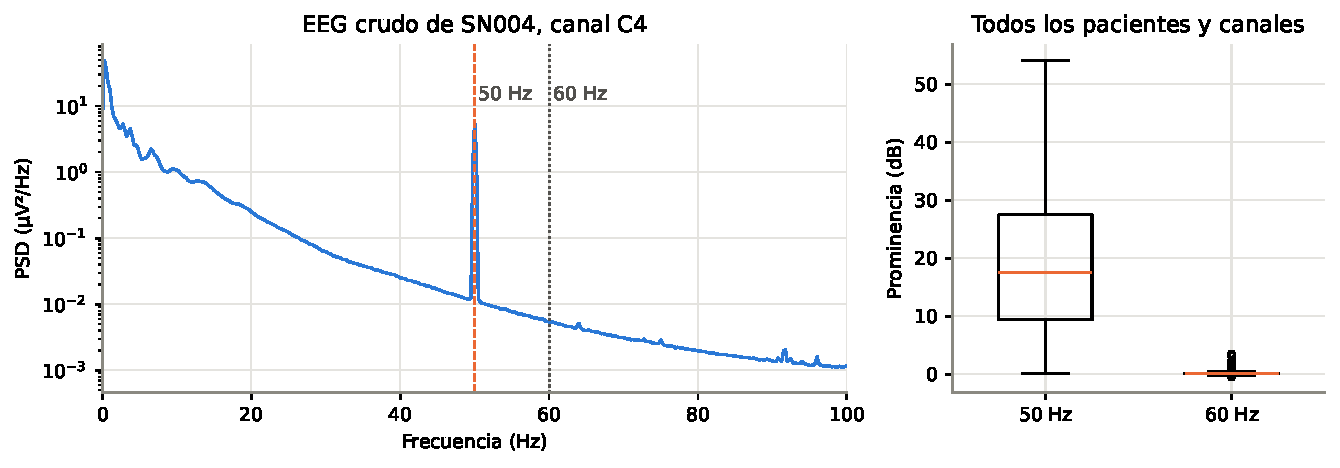
\includegraphics[width=0.9\textwidth]{a_linea_electrica}
  \caption{Espectro crudo de un paciente (izquierda) y prominencia de 50 y \SI{60}{\hertz} en los pacientes de entrenamiento (derecha).}
  \label{fig:linea}
\end{figure}

\textbf{Artefacto ocular.} Corregir toda la noche redujo un 6,5\,\% (Wiener) y un 14\,\% (NLMS) las ondas lentas detectadas en N3. Wiener con compuerta conservó N3 (de 5018 a 4994 ondas, en 12 pacientes) y redujo un 19\,\% las detecciones en REM, que eran movimientos oculares (Fig.~\ref{fig:ondas}). NLMS con compuerta aumentó la potencia delta en W y N1, por lo que se adoptó Wiener.

\begin{figure}[htbp]
  \centering
  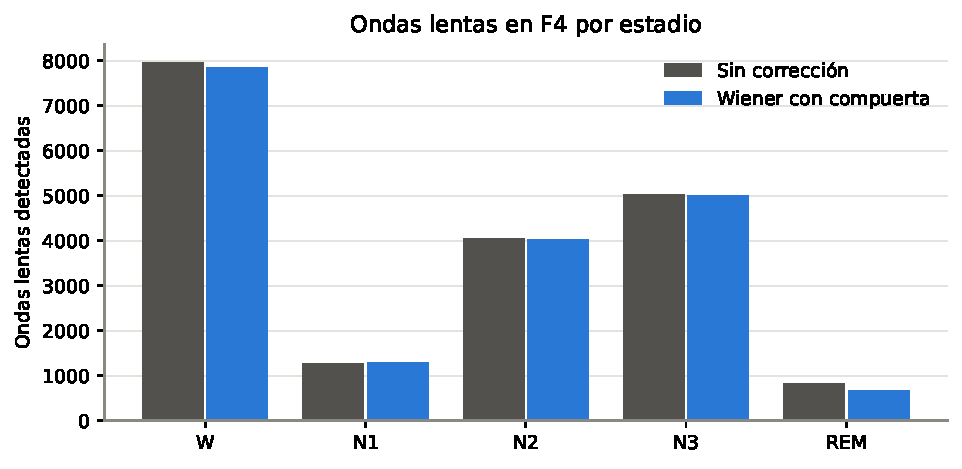
\includegraphics[width=0.6\textwidth]{a_ondas_por_estadio}
  \caption{Ondas lentas detectadas en F4 por estadio, antes y después de la corrección ocular.}
  \label{fig:ondas}
\end{figure}

\textbf{Artefacto cardíaco.} El promedio sincronizado mostró el QRS y la onda T en los 12 pacientes analizados (Fig.~\ref{fig:cardiaco}). En F4 su amplitud mediana fue de \SI{17}{\micro\volt} pico a pico, unas 40 veces la del control con instantes al azar (\SI{0,4}{\micro\volt}), lo que responde a la duda planteada en la devolución. C3, referido a M2, tuvo la mitad de artefacto que los canales referidos a M1. La remoción lo redujo a \SI{1,6}{\micro\volt} (91\,\%) sin cambiar la potencia delta, y quitó más potencia en REM que en W, con \SI{0,55}{\decibel} contra \SI{0,06}{\decibel} en alfa de O2 y \SI{0,62}{\decibel} contra \SI{0,16}{\decibel} en sigma de C4.

\begin{figure}[htbp]
  \centering
  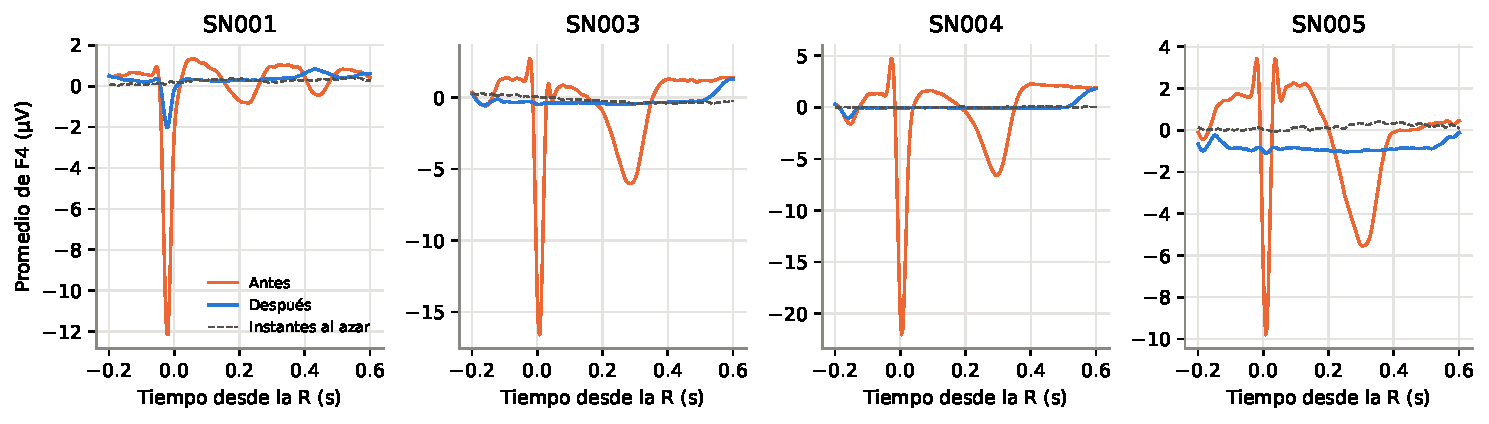
\includegraphics[width=\textwidth]{a_promedio_latidos}
  \caption{Promedio de F4 alrededor de cada latido antes y después de la remoción, y en instantes al azar como control.}
  \label{fig:cardiaco}
\end{figure}

\textbf{Segmentación.} La marca de no estacionariedad abarcó el 10\,\% de las épocas de entrenamiento, con 25\,\% en W y 3\,\% en N3, y fue más frecuente en las épocas de transición entre estadios (17,5\,\% contra 7,5\,\%). En las épocas marcadas el clasificador acertó el 28\,\% contra el 45\,\% de las no marcadas. Un tercio de las épocas marcadas de W, N1, N2 y REM se clasificó como N3, porque la regla de N3 tomó las deflexiones grandes como ondas lentas.

\textbf{Latidos y HRV.} En los 12 pacientes analizados, Pan-Tompkins detectó entre 24\,700 y 37\,900 latidos por noche, con RR medianos entre 0,69 y \SI{1,06}{\second}. El descarte por forma sacó una mediana del 4,9\,\% de los latidos, y después de filtrar los intervalos se conservó al menos el 90\,\% en 10 de los 12 pacientes. La excepción fue SN001, con el 47\,\%, porque tiene un ritmo muy irregular. El 24\,\% de sus intervalos es más de un 20\,\% más corto que el de sus vecinos, contra una mediana del 1,8\,\% en los demás. El cociente LF/HF fue menor en N3 y mayor en REM, como se esperaba, con percentiles medianos de 25 y 70 dentro de la noche. HF bajó en REM pero no subió en N3, por lo que la regla de REM usa el cociente.

\textbf{Descriptores por estadio.} Para ver si cada descriptor separa los estadios en todos los pacientes y no solo en uno, se estandarizó cada descriptor dentro de cada noche y se promedió por estadio en cada uno de los 56 pacientes de entrenamiento, entre luces apagadas y encendidas (Fig.~\ref{fig:huella}). El descriptor más consistente fue la pendiente del espectro, que en C4 pasó de una mediana de $-1{,}36$ en W a $-2{,}66$ en N3 y fue más empinada en N3 que en W en los 56 pacientes. La potencia $\delta$ relativa en F4 fue máxima en N3 en 49 pacientes y la amplitud del EMG fue mínima en REM en 43. La $\alpha$ relativa en O2 fue máxima en W solo en 31, y la energía del EOG resultó más alta en W que en REM ($+0{,}92$ contra $+0{,}46$ desvíos), de modo que ninguno de los dos alcanza por sí solo para reconocer esos estadios.

\begin{figure}[htbp]
  \centering
  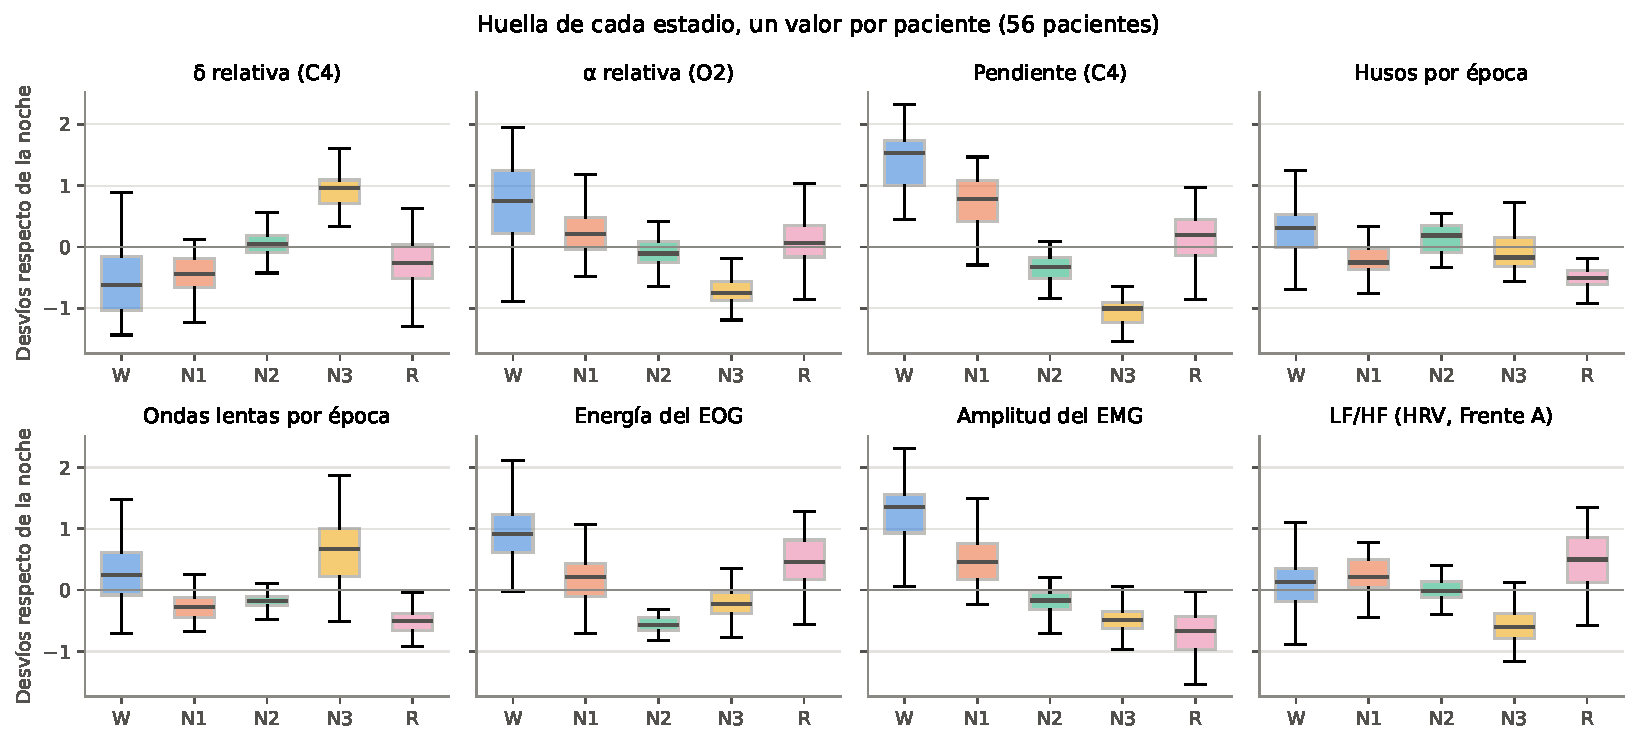
\includegraphics[width=\textwidth]{b_huella_pacientes}
  \caption{Descriptores estandarizados dentro de cada noche, un valor por paciente y por estadio (56 pacientes de entrenamiento). La línea horizontal marca el valor medio de la noche.}
  \label{fig:huella}
\end{figure}

\textbf{Husos y ondas lentas en vigilia.} Los dos detectores encontraron eventos en W. La mediana entre pacientes fue de 1,10 husos por época en W y de 0,99 en N2, y W superó a N2 en 34 de los 56 pacientes. Las ondas lentas fueron 2,42 por época en N3 y 1,79 en W, y N3 superó a todos los demás estadios solo en 33 pacientes. Dentro de W, las épocas con dos o más husos tuvieron un EMG más alto que las que no tenían ninguno en los 56 pacientes (mediana de 17 contra \SI{7}{\micro\volt}) y menos $\alpha$ en O2 en 55 (0,04 contra 0,15). Con las ondas lentas el resultado fue el mismo. En el paciente de ejemplo, además, las detecciones de W tuvieron la misma frecuencia que las de N2, cerca de \SI{13}{\hertz}, y la corrección ocular redujo un 75\,\% las ondas lentas de REM pero solo un 7\,\% las de W. Las detecciones de vigilia corresponden entonces a vigilia activa, con movimiento y tensión muscular, y no al ritmo $\alpha$ ni a movimientos oculares.

\textbf{Woody sobre ondas reales.} En los 55 pacientes de entrenamiento con al menos cinco ondas lentas en N3, la plantilla de Woody tuvo un valle menos profundo que el promedio ordinario (mediana de $-78{,}9$ contra \SI{-83,1}{\micro\volt}), porque cada onda se recorta centrada en su mínimo y el promedio ordinario suma ahí el ruido de todas. El algoritmo convergió antes de las 20 iteraciones en 25 pacientes. En los demás siguió moviendo unas pocas ondas muy deformadas, que saltan entre posiciones sin estabilizarse, y en el paciente mediano el 0,4\,\% de las ondas quedó en el corrimiento máximo de \SI{0,25}{\second}. Entre las épocas con ondas, la similitud con la plantilla fue parecida en todos los estadios (mediana entre 0,74 y 0,79).

\subsection{Clasificación}
\pendiente{Comentar la distribución de estadios (\texttt{c\_distribucion\_estadios}) y los umbrales elegidos (\texttt{c\_eleccion\_umbrales}).}

% \begin{figure}[htbp]
%   \centering
%   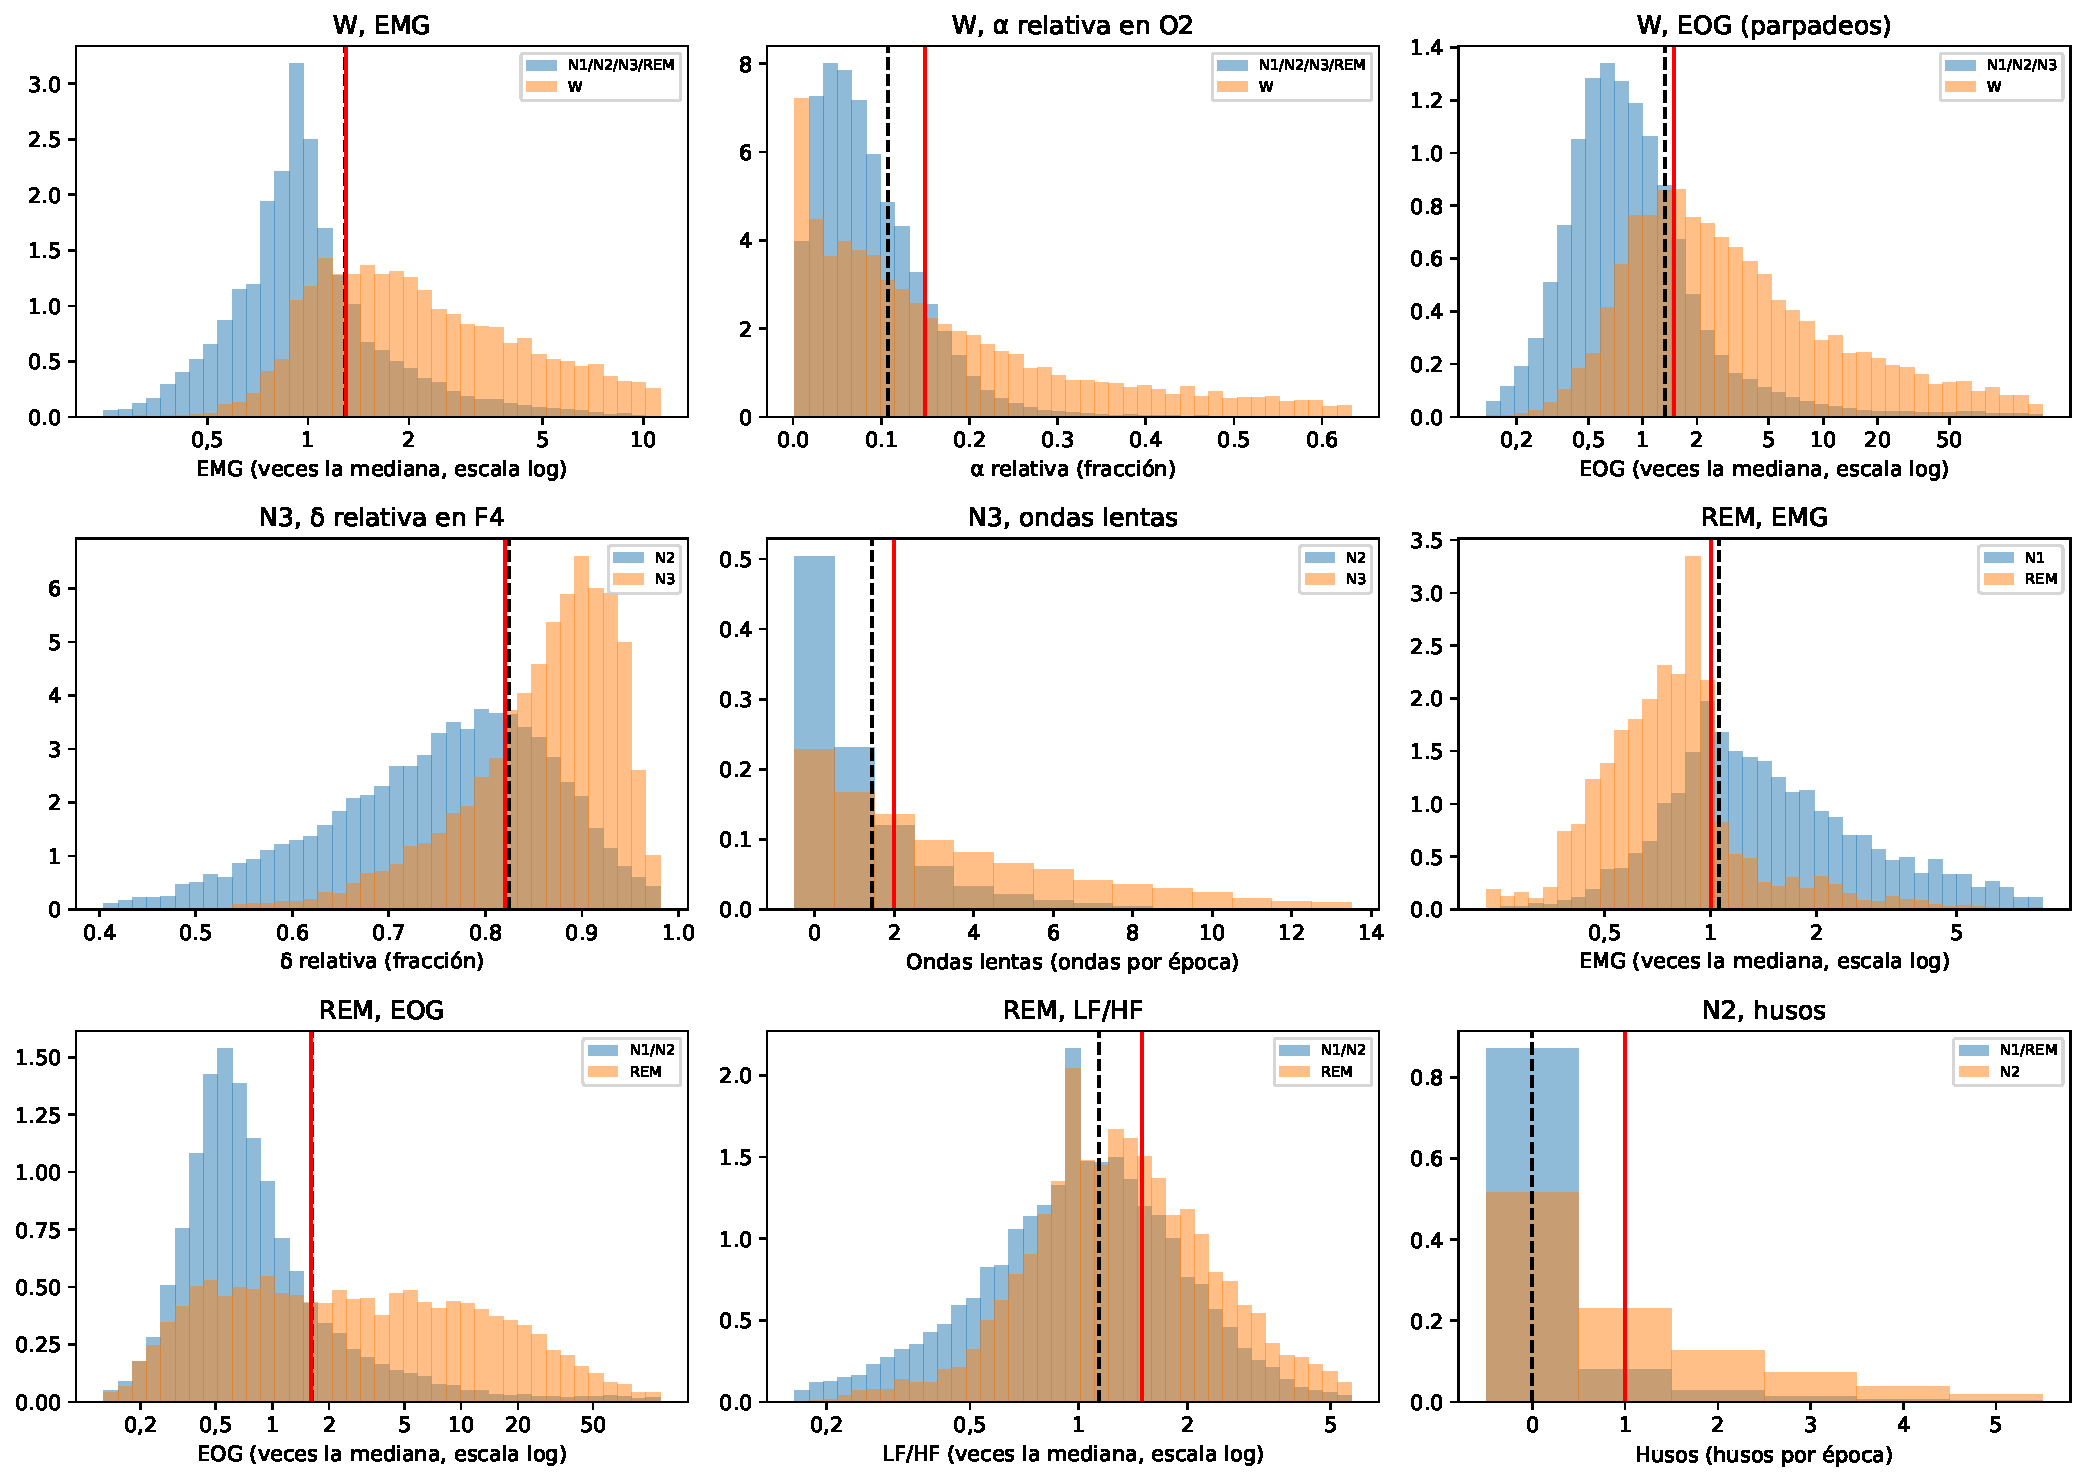
\includegraphics[width=\textwidth]{c_eleccion_umbrales}
%   \caption{Histogramas de cada descriptor en los estadios que separa cada regla (pacientes de entrenamiento). Punteada: cruce de los histogramas; roja: umbral elegido.}
%   \label{fig:umbrales}
% \end{figure}

\begin{table}[htbp]
  \centering
  \caption{Acuerdo con los técnicos sobre los \pendiente{14} pacientes de prueba.}
  \label{tab:resultados}
  \begin{tabular}{lcccccc}
    \toprule
    & $\kappa$ & F1 W & F1 N1 & F1 N2 & F1 N3 & F1 REM \\
    \midrule
    Reglas                  & -- & -- & -- & -- & -- & -- \\
    Reglas + moda           & -- & -- & -- & -- & -- & -- \\
    Reglas + continuidad    & -- & -- & -- & -- & -- & -- \\
    \midrule
    Técnicos HMC~\cite{alvarez2021}        & 0,74 & & & & & \\
    Red de referencia~\cite{alvarez2021}   & 0,79 & & & & & \\
    \bottomrule
  \end{tabular}
\end{table}

% \begin{figure}[htbp]
%   \centering
%   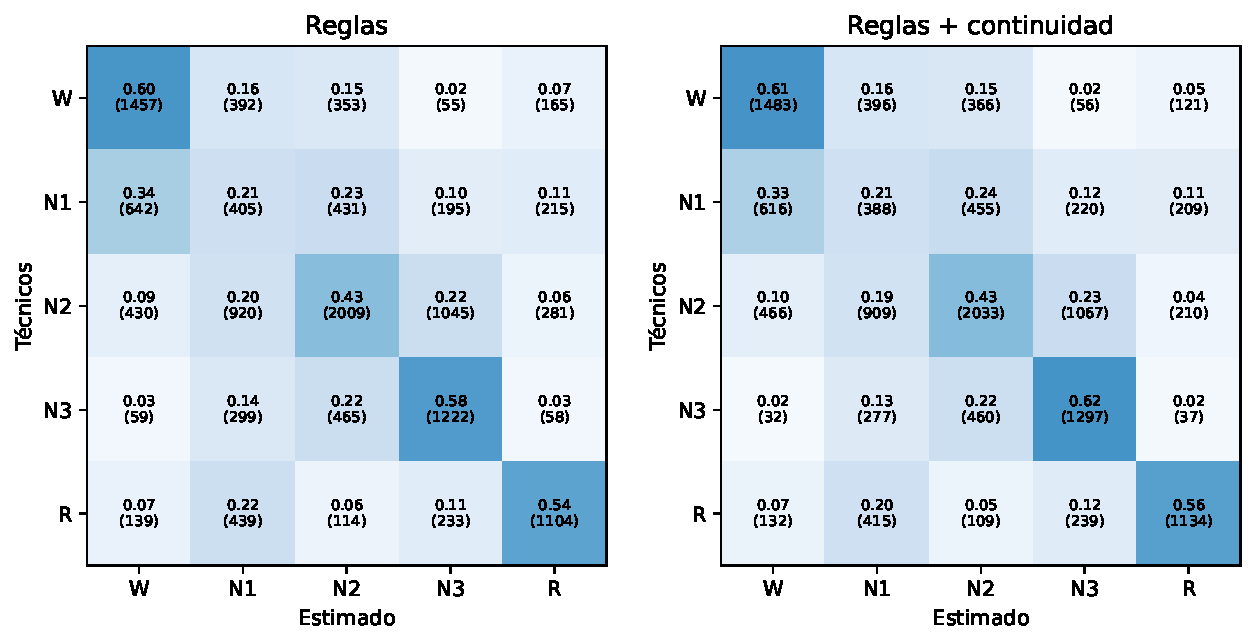
\includegraphics[width=\textwidth]{c_matrices_confusion}
%   \caption{Matrices de confusión normalizadas por fila (estadio de los técnicos).}
%   \label{fig:confusion}
% \end{figure}

% \begin{figure}[htbp]
%   \centering
%   \includegraphics[width=\textwidth]{c_hipnograma_SNxxx}
%   \caption{Hipnograma de un paciente de prueba: técnicos, reglas y reglas con suavizado.}
%   \label{fig:hipnograma}
% \end{figure}

% \begin{figure}[htbp]
%   \centering
%   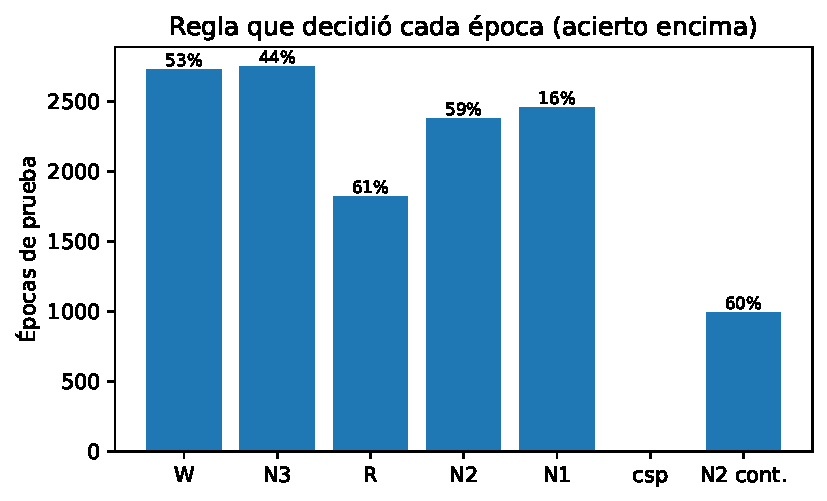
\includegraphics[width=0.7\textwidth]{c_uso_reglas}
%   \caption{Cantidad de épocas de prueba que decidió cada regla y fracción de aciertos.}
%   \label{fig:uso_reglas}
% \end{figure}

\subsection{Verificación de hipótesis}

\begin{table}[htbp]
  \centering
  \caption{Comparaciones paciente por paciente (Wilcoxon).}
  \label{tab:hipotesis}
  \begin{tabular}{llccc}
    \toprule
    & Medida & Variante A & Variante B & $p$ \\
    \midrule
    H1 & Variación por banda     & Multitaper: 0,142 & Welch: 0,148      & 0,0001 \\
       & Variación por frecuencia & Multitaper: 0,182 & Welch: 0,220     & 0,0001 \\
    H2 & Error de forma          & Woody: 0,28      & Promedio: 0,42   & 0,049 \\
    H3 & F1 de N1                & Con desempate: 0,21 & Sin desempate: 0,20 & 0,13 \\
       & F1 de REM               & Con desempate: 0,54 & Sin desempate: 0,58 & 0,033 \\
    H4 & Residuo cardíaco (\si{\micro\volt}) & Después: -- & Antes: -- & -- \\
       & $\kappa$                & Con etapas: -- & Sin etapas: -- & -- \\
    \bottomrule
  \end{tabular}
\end{table}

\section{Discusión}
\textbf{Acuerdo alcanzado.} El clasificador por reglas llegó a $\kappa = 0{,}343$ sobre los pacientes de prueba, lejos del acuerdo entre los técnicos del HMC (0,74) y de la red de referencia (0,79). Es un acuerdo bajo pero claramente superior al azar, y conviene leerlo junto con lo que cada número representa: la red aprende de miles de épocas etiquetadas qué combinación de rasgos separa los estadios, mientras que acá cada estadio se reconoce con dos o tres descriptores y umbrales fijos, que se pueden leer y justificar uno por uno. El $\kappa$ además varió mucho entre pacientes (de 0,16 a 0,55, con mediana 0,28), lo que indica que parte del error depende de la calidad y de las particularidades de cada registro.

\textbf{Dónde se equivoca.} Los errores se concentran en las fronteras que también son difíciles para los técnicos. N1 fue el estadio peor reconocido (F1 de 0,18): se asigna por descarte, de modo que recibe las épocas de cualquier estadio que no cumplen ninguna regla, y solo el 16\,\% de las épocas asignadas así eran realmente N1. La frontera entre N2 y N3 es gradual, porque N3 se define por la proporción de la época ocupada por ondas lentas; esto se vio al elegir el umbral de ondas, donde 2 y 3 dieron casi el mismo acuerdo, uno a costa de N2 y el otro a costa de N3. Por último, las épocas N1 con movimientos oculares y tono muscular conservado se parecen a la vigilia con ojos abiertos, que la regla de W reconoce por los parpadeos.

\textbf{Suavizado.} Las reglas de continuidad mejoraron poco el acuerdo (de 0,330 a 0,343), pero con un balance favorable: por cada error que introdujeron corrigieron 1,4. El filtro de moda cambió casi el doble de épocas con un balance peor, porque también borra tramos cortos reales, como los despertares breves. Que el suavizado aporte poco indica que la mayoría de los errores no son épocas aisladas, sino tramos enteros asignados al estadio equivocado.

\textbf{Reglas frente a LDA + HMM.} Al reemplazar el LDA y el HMM por reglas fijas se resignó parte del acuerdo esperable: un clasificador supervisado pondera todos los descriptores a la vez, mientras que cada regla usa solo dos o tres. A cambio, cada época queda explicada por una regla concreta (Fig.~\ref{fig:uso_reglas}), con umbrales que tienen interpretación fisiológica y que no dependen de un entrenamiento. Esa trazabilidad permitió diagnosticar cada error: la regla de N3 acierta menos (44\,\%) porque cuenta como ondas lentas las deflexiones de los movimientos, y la de N1 casi nunca acierta porque recibe lo que las demás descartan. Una primera versión, que expresaba todos los descriptores como percentiles de la noche, mostró además que normalizar por paciente sin criterio es contraproducente: fijaba la proporción de cada estadio en cada noche y llevaba a N3 épocas de vigilia de pacientes con poco sueño profundo.

\textbf{Preprocesamiento.} Cada parámetro del preprocesamiento salió de una medición sobre los pacientes de entrenamiento, y dos de esas mediciones cambiaron lo que proponía el anteproyecto. El pasa-altos tuvo que bajar a \SI{0,2}{\hertz} para no perder ondas lentas. Y la corrección ocular aplicada a toda la noche borraba ondas lentas reales en N3, porque E1$-$E2 también registra actividad cerebral, lo que obligó a agregar la compuerta. La remoción cardíaca, que la cátedra puso en duda, resultó relevante por un motivo que no era evidente. El artefacto tiene la misma amplitud toda la noche, pero pesa más en REM, donde el EEG es más chico, y sin quitarlo REM se parece más a W y a N2 en las bandas alfa y sigma.

La marca de no estacionariedad mostró una fuente concreta de error del clasificador. Un tercio de las épocas marcadas de W, N1, N2 y REM se clasificó como N3, porque los movimientos y los despertares producen deflexiones grandes y lentas que la regla de N3 cuenta como ondas lentas. Una mejora posible es no asignar N3 a las épocas marcadas, o contar las ondas solo en los tramos estables de la época.

El preprocesamiento tiene cuatro limitaciones. El equipo aplicó un pasa-bajos de \SI{35}{\hertz} en 27 de los 56 pacientes de entrenamiento y de \SI{128}{\hertz} en el resto, lo que puede correr la pendiente espectral de un grupo respecto del otro. SN020 tiene más de un tercio de sus épocas saturadas, y la HRV de SN001 es poco confiable por su ritmo irregular. Por último, en W se siguen detectando ondas lentas que probablemente sean movimientos del cuerpo que el EOG no registra.

\textbf{Descriptores y técnicas no vistas en clase.} H1 se confirmó, porque el multitaper varió menos que Welch entre épocas vecinas de un mismo estadio en los 14 pacientes de prueba (Tabla~\ref{tab:hipotesis}). La mejora fue del 18\,\% al comparar frecuencia por frecuencia, pero solo del 4\,\% al comparar potencias por banda, ya que integrar una banda promedia muchas frecuencias y Welch se acerca así al multitaper. Como los descriptores son potencias por banda, la ventaja del multitaper existe pero es chica para este uso.

H2 se confirmó con un margen estrecho. Con ondas de forma conocida, Woody tuvo menos error que el promedio ordinario en 11 de los 14 pacientes ($p = 0{,}049$). En las ondas reales el promedio ordinario dio un valle más profundo, pero eso no indica una forma más fiel, sino que cada recorte está centrado en su propio mínimo y el ruido se suma justo ahí. Que el algoritmo no haya convergido en más de la mitad de los pacientes sugiere agregar una tolerancia, de modo que termine cuando cambian pocas ondas y no cuando no cambia ninguna. La segunda parte de H2, que Woody ayude a separar N2 de N3, no se sostiene. La similitud con la plantilla es casi igual en todos los estadios, y lo que separa N3 es la cantidad de ondas y no su forma.

H3 no se confirmó. El desempate con CSP mejoró levemente el F1 de N1 (mediana de 0,16 frente a 0,14; fue peor con CSP solo en 5 de los 14 pacientes), sin que la diferencia fuera significativa ($p = 0{,}060$), y empeoró el de REM (0,46 frente a 0,57, peor en 10 de los 14; $p = 0{,}009$), por lo que el clasificador final no lo usa. En un paciente aislado CSP separa N1 de REM, pero los filtros se ajustaron con las covarianzas de los 56 pacientes de entrenamiento juntos, y la combinación de canales que separa los dos estadios cambia de un paciente a otro. Además, la clase N1 que corrige el desempate es la que asignan las reglas por descarte, que mezcla épocas de todos los estadios.

El hallazgo más útil de los descriptores fue la vigilia activa. Las épocas de W con movimiento tienen EMG alto, poca $\alpha$, y también husos y ondas lentas detectados. Sin $\alpha$ no cumplían la regla de W, y terminaban en N3 por las ondas, en N2 por los husos o en N1 por descarte. Por eso la regla final de W acepta, en lugar de la $\alpha$, parpadeos (EOG alto), que recuperan la vigilia con ojos abiertos. La vigilia con movimiento pero sin parpadeos sigue sin reconocerse; una regla que acepte un EMG muy alto aunque falten la $\alpha$ y los parpadeos atacaría ese error restante.

H4 se confirmó solo en parte. La remoción eliminó el artefacto cardíaco en los 14 pacientes de prueba, con un residuo mediano de 1,2~\si{\micro\volt} frente a 19,5~\si{\micro\volt} antes de remover ($p = 0{,}0001$), pero el acuerdo con los técnicos no cambió al quitar los artefactos y la HRV ($\kappa$ mediano de 0,28 con estas etapas y 0,29 sin ellas; fue menor con las etapas en 6 de los 14 pacientes, $p = 0{,}54$). El artefacto existe y la remoción funciona, como mostró también el análisis del preprocesamiento, pero las reglas finales casi no lo perciben: usan potencias relativas sobre épocas de 30~s, en las que un pulso de pocos microvoltios pesa poco, y el EMG y el EOG, que se registran en canales aparte. El cociente LF/HF, por su parte, separó poco REM de N1 y N2. Para este clasificador, entonces, la remoción del artefacto cardíaco no era necesaria, como sugirió la devolución; sí lo sería para descriptores más sensibles a la forma de onda.

\textbf{Limitaciones.} Los umbrales se eligieron con una sola partición en 56 pacientes de entrenamiento y 14 de prueba; con tan pocos pacientes de prueba, el $\kappa$ global depende bastante de cuáles tocaron en cada grupo. Durante el desarrollo, el acuerdo sobre los pacientes de prueba se consultó para descartar la primera versión basada en percentiles y en un ajuste intermedio del umbral de ondas lentas; ese ajuste se revirtió y los umbrales finales se eligieron solo con los pacientes de entrenamiento, pero el resultado de prueba no es completamente independiente del diseño. Por último, en esta base casi no hay épocas fuera del período entre luces apagadas y encendidas, por lo que esa decisión no pudo evaluarse.

\section{Conclusiones}
\pendiente{Conclusiones.}

\textbf{Trabajo futuro.} Para la instancia final, donde sí se permiten técnicas de inteligencia artificial, se propone retomar el esquema del anteproyecto: un LDA sobre los mismos descriptores y un HMM con Viterbi para la corrección temporal, y compararlos con el clasificador por reglas sobre los mismos pacientes de prueba.


\printbibliography

\end{document}
